% SOICT 2026 - Springer CCIS camera-ready (short paper, 8-11 pages incl. references).
%
% Build: pdflatex paper && bibtex paper && pdflatex paper && pdflatex paper

% Camera-ready: the llncs class is used unmodified (A4, default text block),
% as the Springer author instructions require.
\documentclass[runningheads]{llncs}
% llncs sets no paper size, so pdfTeX falls back to Letter; Springer works in A4.
\setlength\paperwidth{210mm}\setlength\paperheight{297mm}

\usepackage[T1,T5]{fontenc}      % T5 for Vietnamese examples
\usepackage[utf8]{inputenc}
\usepackage{graphicx}
\usepackage{booktabs}
\usepackage{enumitem}
\usepackage{amsmath}
\usepackage{multirow}
% microtype off: LNCS Type1 fonts are not scalable, breaks pdfTeX font expansion
\usepackage{tikz}
\usetikzlibrary{arrows.meta,positioning,calc,shapes.geometric,fit,backgrounds,decorations.pathreplacing,shadows,shapes.callouts}
\usepackage{xcolor}
\usepackage{float}     % [H]: ghim float dung cho no xuat hien
\usepackage{placeins}  % \FloatBarrier: giu bang trong section cua no
\usepackage{needspace}  % keep a heading with the lines that follow it
\usepackage{pifont}     % \ding{41}: envelope for the corresponding author
% Links stay navigable but print black: Springer proceedings are printed in
% monochrome, and coloured cross-references look like typos on paper.
\usepackage{hyperref}
\hypersetup{colorlinks=true, linkcolor=black, citecolor=black,
            urlcolor=black, pdfborder={0 0 0}}

% ORCID ids use the class's own \orcidID; Springer typesets the logo.
\newcommand{\envelopeicon}{\ding{41}}
\newcommand{\envelope}{\textsuperscript{\footnotesize\ding{41}}}
% The keyword separator is TS1's \textperiodcentered, which this TeX install has
% only as a bitmap (Type 3) font; Springer asks for outline fonts.
\DeclareTextCommandDefault{\textperiodcentered}{\ensuremath{\cdot}}

% Muted palette; distinguishable in greyscale (brightness differs).
\definecolor{cData}{HTML}{E8EEF7}
\definecolor{cDataL}{HTML}{4A6FA5}
\definecolor{cScore}{HTML}{FDF0E3}
\definecolor{cScoreL}{HTML}{C97B24}
\definecolor{cLLM}{HTML}{EAF3EA}
\definecolor{cLLML}{HTML}{4E8A52}
\definecolor{cLoop}{HTML}{9B4D8C}

\renewcommand{\floatpagefraction}{0.9}
\renewcommand{\topfraction}{0.9}
\renewcommand{\bottomfraction}{0.7}
\renewcommand{\textfraction}{0.08}

\emergencystretch=2em % lets lines with long inline math break instead of overrunning

\begin{document}

\title{Beyond the English Baseline: {IterCOMP-X} for\\Vietnamese Multi-Hop Question Answering}

\titlerunning{Beyond the English Baseline: IterCOMP-X}

\author{Thanh-Nhan Truong\inst{1,2}\textsuperscript{(\envelopeicon)}\orcidID{0009-0007-5012-7578} \and
Ngoc-Vy Tran\inst{1,2}\orcidID{0009-0003-6339-7543} \and
Nhat-Minh Tran\inst{1,2}\orcidID{0009-0005-8677-1897}}

\authorrunning{T.-N. Truong et al.}

\institute{Faculty of Information Technology, University of Science,
Ho Chi Minh City, Vietnam\\
\email{$\{$25C1505320, 25C1506947, 24C11055$\}$@student.hcmus.edu.vn}
\and
Vietnam National University, Ho Chi Minh City, Vietnam}

\maketitle
\begin{abstract}
Training-free prompt compressors are developed and evaluated almost entirely on
English. We reimplement the iterative compressor IterCOMP as IterCOMP-X, leaving
its algorithm unchanged, and contribute its first evaluation on Vietnamese
multi-hop question answering together with the measurements that evaluation
requires. On VimQA and three English datasets, read by a 4-bit Qwen2.5-7B,
IterCOMP-X retains 0.19 to 0.35 of the tokens and outperforms the token-level
LLMLingua-2 by 10.72 to 18.58 F1, a lead that survives matched retention but
narrows under a second reader. The accuracy is paid for in latency: repeated
judge calls make it 3.2 to 7.2 times slower than LLMLingua-2. Its gain over the
uncompressed context concentrates on questions whose evidence spans two
documents, and it keeps 91\% of the gold evidence, so most of its misses are
the reader's. Retention itself is not
comparable across languages: Vietnamese costs 2.39 times as many billed tokens as
English for the same content, so we report an effective ratio that prices
retention in English-equivalent tokens. Boolean-answer normalisation is worth
8.67 F1 on Vietnamese and nothing in English, and removing diacritics costs about 20 F1 in gold and compressed contexts alike, mostly in the reader, while lowering gold-evidence recall by 6 points.

\keywords{Prompt Compression \and Multi-Hop Question Answering \and
\mbox{Tokeniser Fertility} \and Vietnamese NLP}
\end{abstract}

\section{Introduction}
Multi-hop question answering aggregates evidence across documents.
Retrieval-augmented generation \cite{lewis2020rag} supplies them at two costs:
input length grows with their number, and irrelevant passages degrade reader
accuracy. Prompt compression addresses both
\cite{jiang2023llmlingua,li2023selectivecontext,pan2024llmlingua2,xu2024recomp},
but usually decides once, conditioned on the original question. That misses what
defines multi-hop QA: evidence for a later hop becomes identifiable only once the
earlier hop's is in. IterCOMP \cite{yun2026itercomp} embeds that reasoning into
the compression loop (Fig.~\ref{fig:arch}), but releases no implementation and
is evaluated only on English.

\begin{figure}[H]
\centering
\resizebox{\textwidth}{!}{%
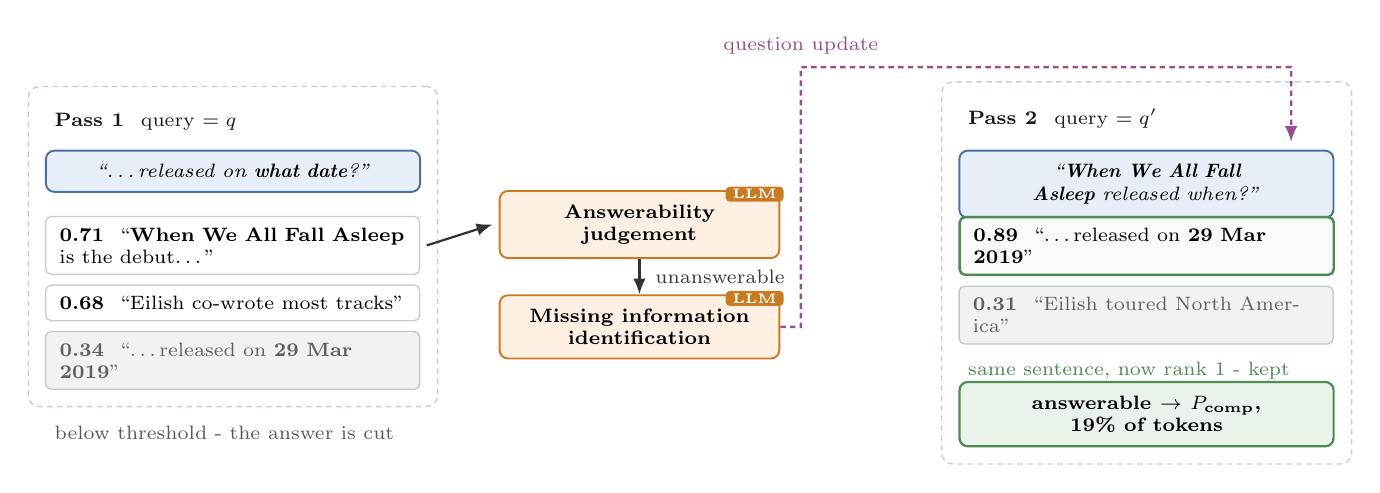
\begin{tikzpicture}[
  font=\footnotesize, x=1cm, y=1cm,
  % ── mot bang mau duy nhat: xanh = du lieu, cam = LLM, luc = ket qua ──
  qq/.style={rounded corners=3pt, draw=cDataL, fill=cData, line width=0.7pt,
             align=center, font=\scriptsize, text width=44mm,
             inner xsep=5pt, inner ysep=5pt},
  sg/.style={rounded corners=2pt, draw=gray!40, fill=white, line width=0.5pt,
             align=left, font=\scriptsize, text width=44mm,
             inner xsep=5pt, inner ysep=4pt},
  kp/.style={sg, draw=cLLML, fill=cLLM!40, line width=0.9pt},
  dp/.style={sg, draw=gray!45, fill=gray!10, text=gray!75!black},
  ai/.style={rounded corners=3pt, draw=cScoreL, fill=cScore, line width=0.7pt,
             align=center, font=\scriptsize\bfseries, text width=32mm,
             inner xsep=5pt, inner ysep=5pt},
  ok/.style={rounded corners=3pt, draw=cLLML, fill=cLLM, line width=0.8pt,
             align=center, font=\scriptsize\bfseries, text width=44mm,
             inner xsep=5pt, inner ysep=5pt},
  tag/.style={font=\tiny\bfseries, text=white, fill=cScoreL, rounded corners=1.5pt,
              inner xsep=2.5pt, inner ysep=1pt},
  a/.style={-{Latex[length=2mm,width=1.6mm]}, line width=0.8pt, gray!40!black},
  b/.style={-{Latex[length=2mm,width=1.6mm]}, line width=0.9pt, cLoop,
            dashed, dash pattern=on 2pt off 1.5pt},
  hd/.style={font=\scriptsize\bfseries, text=gray!20!black, anchor=west},
  nt/.style={font=\scriptsize, align=left, anchor=north west},
]
% ═══ luoi: cot x = 0 / 6.4 / 10.6 ; hang y cach deu 0.72 ═══
% Column anchors. The gap between the evidence boxes (44mm wide, left-aligned
% at \cL) and the LLM column has to clear the arrowheads, or they render as
% stubs; \cM and \cR are spaced for that, not packed.
\def\cL{0}      \def\cM{7.55}   \def\cR{11.60}

% ── PASS 1 ───────────────────────────────────────────────
\node[hd] (h1) at (\cL,2.86) {Pass 1 \ \textnormal{query $=q$}};
\node[qq, anchor=north west] (q1) at (\cL,2.50)
  {\emph{``\dots released on \textbf{what date}?''}};
\node[sg, anchor=north west] (s1) at (\cL,1.66)
  {\textbf{0.71} \ ``\textbf{When We All Fall Asleep} is the debut\dots''};
\node[sg, anchor=north west] (s2) at ($(s1.south west)+(0,-0.12)$)
  {\textbf{0.68} \ ``Eilish co-wrote most tracks''};
\node[dp, anchor=north west] (s3) at ($(s2.south west)+(0,-0.12)$)
  {\textbf{0.34} \ ``\dots released on \textbf{29 Mar 2019}''};
% This label sits below the last box; \path reserves the strip it needs so
% resizebox does not scale it off the bottom edge.
% The caption sits outside the dashed group, so it needs clearance below the
% frame edge (which extends inner sep=6pt past s3) rather than below s3 itself.
\node[nt, text=gray!70!black, anchor=north west] at ($(s3.south west)+(0,-0.34)$)
  {below threshold - the answer is cut};
\path ($(s3.south west)+(0,-0.80)$);

% ── LLM ──────────────────────────────────────────────────
\node[ai] (j1) at (\cM,1.55) {Answerability\\ judgement};
\node[tag, anchor=north east] at ($(j1.north east)+(0.05,0.05)$) {LLM};
\node[ai] (j2) at (\cM,0.25) {Missing information\\ identification};
\node[tag, anchor=north east] at ($(j2.north east)+(0.05,0.05)$) {LLM};
\draw[a] ($(s1.east)+(0.08,0)$) -- ($(j1.west)+(-0.08,0)$);
\draw[a] (j1) -- node[font=\scriptsize, right=2pt, text=gray!45!black]
         {unanswerable} (j2);

% ── PASS 2 ───────────────────────────────────────────────
\node[hd] (h2) at (\cR,2.90) {Pass 2 \ \textnormal{query $=q'$}};
\node[qq, anchor=north west] (q2) at (\cR,2.50)
  {\emph{``\textbf{When We All Fall Asleep} released when?''}};
% Two-line boxes need more than the 0.66 step the one-line boxes use, or they
% overlap; the evidence rows are stacked below each other explicitly instead.
\node[kp, anchor=north west] (t1) at (\cR,1.66)
  {\textbf{0.89} \ ``\dots released on \textbf{29 Mar 2019}''};
\node[dp, anchor=north west] (t2) at ($(t1.south west)+(0,-0.12)$)
  {\textbf{0.31} \ ``Eilish toured North America''};
\node[nt, text=cLLML, anchor=north west] at ($(t2.south west)+(0,-0.10)$)
  {same sentence, now rank 1 - kept};
\node[ok, anchor=north west] (rd) at ($(t2.south west)+(0,-0.46)$)
  {answerable $\rightarrow$ $P_\text{comp}$, 19\% of tokens};

% ── vong lap: di vong LEN TREN, khong cat qua hop nao ──
% The loop arrow enters q2 from the left rather than from above: the Pass 2
% heading sits just over the box, and a vertical entry crosses the q' glyph.
% One clean detour: right out of the LLM column, up over the gap, across, then
% down into q2. The descent is offset to q2's right so it misses the "query = q'"
% heading, which sits directly above the box's centre.
% Drawn leg by leg rather than with |- / -|: those operators pick their own
% corner, which here lands a stray vertical stub in the gap between columns.
\draw[b] (j2.east) -- (9.60,{0.25})
         -- (9.60,3.55)
         -- ($(q2.north east)+(-0.55,3.55-2.50)$)
         -- ($(q2.north east)+(-0.55,0.10)$);
\node[font=\scriptsize, text=cLoop, anchor=south] at (9.60,3.59)
  {question update};

\begin{scope}[on background layer]
% The group frames include the pass headings: sized to the boxes alone, the
  % dashed border lands on the heading baseline and strikes through it.
  \node[fit=(h1)(q1)(s1)(s2)(s3), draw=cDataL!35, dashed, line width=0.5pt,
        dash pattern=on 2pt off 1.6pt, rounded corners=4pt, inner sep=6pt] {};
  \node[fit=(h2)(q2)(t1)(t2)(rd), draw=cLLML!35, dashed, line width=0.5pt,
        dash pattern=on 2pt off 1.6pt, rounded corners=4pt, inner sep=6pt] {};
\end{scope}
\end{tikzpicture}}
\caption{A bridge question through two IterCOMP passes, in English for
legibility. The sentence carrying the release date scores $0.34$ against the
original question and is filtered out; re-scored against the follow-up $q'$ it
rises to $0.89$ and is kept.}
\label{fig:arch}
\end{figure}

Transferring it raises questions an English benchmark cannot ask. Vietnamese
marks tone with diacritics that informal text omits, answers polar questions
with a word sharing no surface form with \emph{yes}, and is split far more finely
than English by the subword vocabularies commercial APIs bill on, so two systems
reporting the same retention do not achieve the same saving.

We separate what we inherit from what we add. \emph{Inherited unchanged}: the
compression loop, its dual-aspect scorer, percentile filter, answerability-based
stopping and hyperparameters. \emph{Ours}:
\begin{itemize}[leftmargin=1.2em,itemsep=0pt,topsep=2pt,parsep=0pt]
\item an open reimplementation, IterCOMP-X, with prompts written for a bilingual
  setting, and the first evaluation of an iterative compressor on Vietnamese
  multi-hop QA, with latency reported next to retention;
\item an \emph{effective ratio} that makes compression ratios comparable across
  languages, correcting a nominal ratio that understates Vietnamese cost by
  $2.39\times$ (Section~\ref{sec:fertility});
\item two Vietnamese-specific measurements: a question-gated boolean
  normalisation worth $+8.67$ F1 on Vietnamese and $0.0$ in English, and the
  first evaluation on non-diacritic text (Section~\ref{sec:vnfindings});
\item an analysis of where compression gains over the uncompressed context
  and where it fails (Section~\ref{sec:loss}).
\end{itemize}
The contribution is therefore one of evaluation and measurement, not a new
compression algorithm.

\section{Related Work}
\emph{Prompt compression} is extractive or abstractive
\cite{li2025promptcompression}. LLMLingua \cite{jiang2023llmlingua} drops tokens
by perplexity, LongLLMLingua \cite{jiang2024longllmlingua} adds query
awareness, LLMLingua-2 \cite{pan2024llmlingua2} recasts it as multilingual token
classification, and Selective-Context \cite{li2023selectivecontext} removes
redundant units; RECOMP \cite{xu2024recomp} also regenerates shorter text. All
compress in one pass. \emph{Iterative methods} such as Self-Ask
\cite{press2023selfask}, IRCoT \cite{trivedi2023ircot}, ReAct
\cite{yao2023react} and HippoRAG \cite{gutierrez2024hipporag} loop over retrieval
or reasoning to expand the context; CompAct \cite{yoon2024compact} and IterCOMP
loop to shrink it. All are evaluated on English.

\emph{Tokeniser disparity} is well documented: \cite{ahia2023allcost} price it
against commercial APIs, \cite{somide2026african} extend it to context capacity,
and \cite{petrov2023tokenizers} frame it as unfairness. Compression work
controls for it, if at all, by matching budgets in the target tokeniser
\cite{lukauskas2026lost}; what is missing is a reported quantity that carries
the correction. For \emph{Vietnamese}, PhoBERT \cite{nguyen2020phobert} and ViT5
\cite{phan2022vit5} serve the language at the model level and VimQA
\cite{le2022vimqa} provides multi-hop QA in the HotpotQA format. XProvence
\cite{mohamed2026xprovence} prunes context in over 100 languages, Vietnamese
among them, but on single-hop QA without per-language retention.

\section{Method}
\subsection{Iterative Multi-Hop Compression (Inherited)}
Given a question $q$ and documents $D$ split into sentence segments $e$, a frozen
bge-m3 encoder \cite{chen2024bgem3} scores each segment with a dense and a sparse
lexical signal,
\begin{equation}
S_{\text{dual}}(q,e) = \lambda\, E(q)^\top E(e) + (1-\lambda)
\sum_{t \in \mathcal{V}(q)\cap\mathcal{V}(e)} w_t^{q}\, w_t^{e},
\end{equation}
and keeps the segments at or above the $k$-th percentile of that question's
scores, $E_{\text{cand}}=\{e \mid S_{\text{dual}}(q,e)\ge
\mathrm{Percentile}(\mathcal{S},k)\}$. The reader then judges whether the
gathered evidence answers $q$; on a negative verdict it writes one follow-up
question $q'$ naming what is missing, and the next pass scores the still
unselected segments against $q'$. Selected segments accumulate and are emitted in
selection order. The loop stops on a positive verdict or at \texttt{max\_iter}; we add a
safeguard absent from the original that also stops it once the evidence passes
$60\%$ of the source, since a judge that never reports sufficiency would
otherwise keep nearly everything. The original prompts are
unpublished; ours constrain the verdict to \texttt{ANSWERABLE\_YES/NO} and read
it by substring, so the judgement never depends on a Vietnamese affirmative (on
150 VimQA questions the reader complied every time).

\subsection{Adaptation to Vietnamese (Ours)}
No model is replaced: bge-m3, LLMLingua-2 and Qwen2.5 are multilingual. The
changes sit in text handling. Tokenisation is Unicode-aware, answer normalisation
keeps diacritics (stripping them merges \emph{má}, \emph{mà}, \emph{mã}), and a
boolean step maps an English \emph{yes/no} to \emph{đúng/không} only when the
\emph{question} closes with the polar frame \emph{phải không/đúng không}. It never
reads the gold answer, so it is available at inference and cannot turn a wrong
answer right. We run no word segmenter, so lexical matching works on syllables.

\subsection{Tokeniser Fertility and the Effective Ratio (Ours)}
\label{sec:fertility}
A compression ratio is read as a saving, which assumes the counted unit costs the
same everywhere. IterCOMP reports a token share without naming the
tokeniser; we count with \texttt{\textbackslash w+}, under
which Vietnamese runs $1.34\times$ English; billing tokenisers do not
(Table~\ref{tab:fertility}). Let $\text{Ratio}_{\text{nom}} =
|P_{\text{comp}}|_{\mathcal{T}} / |D|_{\mathcal{T}}$ for a counter
$\mathcal{T}$, and let $\phi_{\mathcal{T}}(\mathcal{L})$ be the mean per-pair
ratio $|x_{\mathcal{L}}|_{\mathcal{T}}/|x_{\text{en}}|_{\mathcal{T}}$ over a
parallel corpus. We report
\begin{equation}
\text{Ratio}_{\text{eff}} = \text{Ratio}_{\text{nom}} \cdot \phi_{\mathcal{T}}(\mathcal{L}),
\label{eq:effratio}
\end{equation}
the cost of the compressed context against an English original of the same
content. The arithmetic is a single factor; the point is to report it, since a
nominal ratio hides the factor entirely. Fixing the IterCOMP-X output on 50
VimQA questions and changing only the tokeniser, the nominal ratio moves within
$1.02\times$ ($0.236$, $0.240$, $0.234$ under \texttt{cl100k\_base},
\texttt{o200k\_base}, \texttt{\textbackslash w+}) while the billed cost moves
$1.58\times$.

\begin{table}[H]
\centering
\caption{Fertility over 930 parallel English-Vietnamese WMT24++ pairs
\cite{deutsch2025wmt24pp}, mean of per-pair ratios; all 95\% intervals are within
$\pm0.04$. OpenAI tokenisers via \texttt{tiktoken} \cite{openai2024tiktoken}.}
\label{tab:fertility}
\small
\begin{tabular}{lrrr}
\toprule
Tokeniser & Vi tok & En tok & Fertility \\
\midrule
\texttt{cl100k\_base} (GPT-4) & 105.6 & 44.1 & \textbf{2.39}$\times$ \\
\texttt{o200k\_base} (GPT-4o) & 63.3 & 43.3 & 1.49$\times$ \\
Qwen2.5 (our reader) & 60.2 & 43.3 & 1.42$\times$ \\
XLM-R (bge-m3) & 57.9 & 49.7 & 1.19$\times$ \\
\texttt{\textbackslash w+} (unit of ``ratio'') & 47.6 & 35.7 & 1.34$\times$ \\
\bottomrule
\end{tabular}
\end{table}

The factor depends on the corpus it is estimated on. WMT24++ is news; rescaling
by the tokens-per-word of Wikipedia text gives $\phi\approx2.01$, and on the
evaluated VimQA contexts themselves \texttt{cl100k\_base} spends $2.13$ tokens per
\texttt{\textbackslash w+} unit. VimQA's effective retention therefore lies
between $0.41$ and $0.49$ depending on the estimate, against a nominal $0.21$; we
report the parallel-corpus value, $0.491$, because VimQA has no English side.

\section{Experimental Setup}
\label{sec:setup}
We evaluate the development sets of HotpotQA \cite{yang2018hotpotqa}, 2Wiki
\cite{ho2020constructing} and MuSiQue \cite{trivedi2022musique}, the original
paper's datasets, at $n=1{,}500$ each, and all $1{,}003$ questions of VimQA, in
the distractor setting (10 passages; 20 for MuSiQue). Smaller analyses use
prefixes of the same splits in file order. We keep the original hyperparameters,
set there with a LLaMA-3-8B reader \cite{grattafiori2024llama3}:
$\texttt{max\_iter}=5$, $\lambda=0.6$, $k=90$ ($85$ for 2Wiki; VimQA takes
HotpotQA's $90$). Re-tuning for Vietnamese is not supported by the data: on VimQA
at $n=500$ no tested $k$ from $70$ to $95$ separates from another. One model,
Qwen2.5-7B \cite{qwen2025qwen25} at 4-bit NF4 on a Tesla T4, is reader and judge,
decoding greedily to 48 tokens.

Raw Documents concatenates all passages; Oracle keeps the gold supporting
sentences (the original keeps whole gold documents), a reference for selection
quality rather than a per-question bound.
LLMLingua-2 is the main baseline, run from its multilingual BERT-base
checkpoint, the only compressor that meets
Vietnamese on equal terms; LLMLingua, LongLLMLingua, Selective-Context, RECOMP
(two forms) and CompAct run on VimQA at $n=200$ but carry English-only
components. R2C has no public checkpoint.

\emph{Metrics.} \emph{F1} is the token overlap between prediction and gold
answer under the HotpotQA normalisation, which keeps Vietnamese diacritics; EM
orders the methods identically and is omitted. \emph{F1$^*$} is F1 after the
boolean normalisation of Section~\ref{sec:vnfindings}. \emph{Retention}
($\text{Ratio}_{\text{nom}}$) is the share of the source context kept, counted in
\texttt{\textbackslash w+} units (the original reports a token share without
naming its tokeniser), and
$\text{Ratio}_{\text{eff}}$ prices it in English-equivalent
\texttt{cl100k\_base} tokens (Eq.~\ref{eq:effratio}). \emph{Latency} (s/q) is
end-to-end wall-clock time per question, compression and reading together.
\emph{Gold-evidence recall} is the share of annotated supporting sentences kept
in $P_{\text{comp}}$, and \emph{coverage} the share of questions that keep all
of them. Differences are paired over the same questions; a $^\dag$ marks a 95\%
paired bootstrap interval (10,000 resamples) that excludes zero.

\section{Results}
\label{sec:results}
\subsection{Accuracy and Cost}
IterCOMP-X outperforms LLMLingua-2 by $+10.72$ to $+18.58$ F1 on all four sets
(Table~\ref{tab:4ds}), every interval clear of zero. The margin is not bought with
a larger budget: on VimQA and HotpotQA IterCOMP-X keeps \emph{fewer} tokens, and
re-running LLMLingua-2 at IterCOMP-X's retention leaves it behind by $+8.22$ F1 on
MuSiQue, CI $[+2.59,+13.99]$, and $+16.79$ on 2Wiki, CI $[+9.90,+23.78]$
($n=200$). On VimQA at $n=200$ it also leads the six further baselines ($50.08$
against $31.22$ down to $7.06$).

\begin{table}[t]
\centering
\caption{Main results, Qwen2.5-7B at 4-bit. F1$^*$ applies the boolean
normalisation of Section~\ref{sec:vnfindings} to every row; it is inert on English.
$\Delta$ is IterCOMP-X minus the baseline, $^\dag$ a paired bootstrap interval
clear of zero. Ratio rows are IterCOMP-X's retention; s/q is end-to-end
wall-clock seconds per question on one T4.}
\label{tab:4ds}
\footnotesize
\setlength{\tabcolsep}{4pt}
\begin{tabular}{lrrrr}
\toprule
F1$^*$ & VimQA & MuSiQue & 2Wiki & HotpotQA \\
$n$ & 1{,}003 & 1{,}500 & 1{,}500 & 1{,}500 \\
\midrule
Oracle & 61.03 & 44.90 & 57.65 & 71.40 \\
Raw & 46.87 & 21.16 & 35.72 & \textbf{59.24} \\
IterCOMP-X & \textbf{51.29} & \textbf{25.35} & \textbf{36.72} & 54.58 \\
LLMLingua-2 & 35.31 & 14.63 & 19.24 & 36.00 \\
\midrule
$\Delta$ vs.\ Raw & $+4.42^\dag$ & $+4.19^\dag$ & $+1.00$ & $-4.66^\dag$ \\
$\Delta$ vs.\ LLMLingua-2 & $+15.98^\dag$ & $+10.72^\dag$ & $+17.48^\dag$ & $+18.58^\dag$ \\
\midrule
Ratio$_\text{nom}$ / Ratio$_\text{eff}$ & 0.206 / 0.491 & 0.340 & 0.354 & 0.194 \\
\midrule
s/q: Raw & 2.88 & 2.65 & 1.15 & 1.67 \\
s/q: LLMLingua-2 & 1.43 & 1.21 & 0.69 & 0.98 \\
s/q: IterCOMP-X & 4.52 & 8.73 & 3.80 & 3.30 \\
\bottomrule
\end{tabular}
\end{table}

\emph{The cost is latency.} Each pass calls the 7B judge once more, and a
negative verdict once more to write $q'$, so IterCOMP-X is $3.2$ to $7.2\times$
slower than LLMLingua-2 and $1.6$ to $3.3\times$ slower than reading everything,
slowest on MuSiQue with its 20 passages. Its saving is in the tokens a metered
reader is billed for, not in time on a local GPU; and those judge calls read the
accumulating evidence too, so retention counts the final reader's input only.

Against Raw the picture is mixed: IterCOMP-X leads on VimQA and MuSiQue, ties on
2Wiki and trails on HotpotQA, where Raw is $4.66$ F1 ahead. Oracle/Raw, the
headroom perfect selection offers, is $2.12$ on MuSiQue, $1.61$ on 2Wiki, $1.30$
on VimQA and only $1.21$ on HotpotQA: a reader that copes with distractors
leaves compression little to recover. Substituting the reader confirms this
(Table~\ref{tab:readers}). A 0.5B reader reverses the HotpotQA loss, and with the
judge pinned at 7B IterCOMP-X leads Raw by $+5.70$, CI $[+1.90,+9.63]$, at $0.192$
retention. Mistral-7B, from another family, preserves the ordering but narrows
the lead over LLMLingua-2 to $+4.42$ with an interval spanning zero, so the
margin over token-level compression should not be read as reader-independent.

\begin{table}[H]
\centering
\caption{Reader substitutions, each a separate run with the reader as its own
judge; $^\dag$ marks a paired bootstrap interval clear of zero.}
\label{tab:readers}
\small
\setlength{\tabcolsep}{5pt}
\begin{tabular}{llrrrr}
\toprule
Reader & Data & $n$ & Ratio$_\text{nom}$ & $\Delta$ vs.\ Raw & $\Delta$ vs.\ LLML-2 \\
\midrule
Qwen2.5-7B    & HotpotQA & 1,500 & 0.194 & $-4.66^\dag$  & $+18.58^\dag$ \\
Qwen2.5-0.5B  & HotpotQA & 500   & 0.532 & $+7.66^\dag$  & $+16.36^\dag$ \\
Qwen2.5-7B    & VimQA    & 200   & 0.193 & $+5.92^\dag$  & $+11.78^\dag$ \\
Mistral-7B    & VimQA    & 200   & 0.182 & $+23.36^\dag$ & $+4.42$ \\
\bottomrule
\end{tabular}
\end{table}

The reimplementation is consistent with the original where it can be checked.
The Oracle/Raw headroom on MuSiQue is $2.12$ against the original's $1.88$, a
loose check since our Oracle keeps gold sentences and theirs gold documents; at
matched retention
($k=96$, $0.160$ against their $0.14$, $n=200$) IterCOMP-X scores $29.04$ F1
against the original $27.36$. Absolute numbers remain incomparable: reader and
prompts differ.

\subsection{Where Compression Gains and Where It Fails}
\label{sec:loss}
\emph{Gains concentrate on multi-document questions.} Splitting VimQA by the
number of documents holding gold evidence, IterCOMP-X ties Raw on the $377$
questions answerable from one document ($+0.86$, CI $[-2.37,+4.00]$) and leads by
$+6.57$, CI $[+2.64,+10.52]$, on the $626$ that need two, the case the loop
targets. Iterating matters less than this suggests: one pass against five gives
$31.73$ against $36.07$ F1 (unnormalised) at $n=500$, inside the $6.6$-point detection
threshold, and the loop stops after $1.58$ passes on average.

\emph{Evidence is rarely what is missing.} On the first $500$ VimQA questions,
$P_{\text{comp}}$ keeps $91.0\%$ of the gold sentences, and all of them for
$83.0\%$ of questions, where IterCOMP-X scores $52.5$ F1 against $23.0$ on the
rest. Of the $67$ questions that gold context answers and IterCOMP-X misses,
only $29$ lack a gold sentence; on the other $38$ the reader fails with the
answer in its context, among the distractor sentences gold context does not
carry. A hand check of $50$ IterCOMP-X predictions agrees: Oracle, given exactly
the gold sentences, still reaches only $61.03$ F1, so $80\%$ of IterCOMP-X's error
persists under perfect retrieval; one error in ten is a yes/no answer right in
substance and wrong in surface form (\emph{tức là yes} for \emph{đúng}), and the
age-comparison template (``is $X$ older than $Y$?'', $9.8\%$ of VimQA) fails as
arithmetic rather than retrieval. Other surface misses: \emph{3} for the gold
\emph{ba} (three), \emph{Spain} for \emph{Tây Ban Nha}. When evidence is lost, an
early stop loses it: $77$ of the $85$ questions missing a gold sentence ended
after one pass. Asked how many Oscars the film in which Dustin Hoffman played a
criminal won, the first pass keeps the sentence naming \emph{Midnight Cowboy},
the judge declares the evidence sufficient, and the answer sentence (``the film
won 3 Oscars''), which names neither film nor actor, is never reached; the
reader answers \emph{unknown}. Asked for the role that made Carole Lombard's
husband famous, the loop again stops at the bridge and the reader returns the
husband. With recall already high, recovering the rest buys little. Pulling in each
kept sentence's neighbours ($\pm1$ in the same document) raises recall by $2.1$
points, CI $[+1.0,+3.3]$, and coverage by $3.4$, CI $[+1.4,+5.4]$, but retention
grows from $0.193$ to $0.276$ and F1$^*$ moves by only $+1.15$, CI
$[-1.59,+3.84]$. Asking the judge to name the bridge entity in $q'$ and adding
the best sentences of any document whose title $q'$ names changes neither recall
($+0.17$) nor F1$^*$ ($-0.55$, CI $[-1.71,+0.55]$).

\subsection{Effects Specific to Vietnamese}
\label{sec:vnfindings}
\emph{Boolean normalisation} adds $+8.67$ F1 to IterCOMP-X on VimQA, CI
$[+6.98,+10.47]$, $+3.99$ to Raw, and exactly $0.0$ on every English set. Asked a
Vietnamese polar question, the reader often answers in English: $12.3\%$ of the
time from IterCOMP-X's context against $3.3\%$ from Raw under Qwen, and $89.6\%$
against $35.8\%$ under Mistral. Without the step IterCOMP-X and Raw are level
($42.61$ against $42.88$, CI $[-2.80,+2.27]$), so its lead over Raw in
Table~\ref{tab:4ds} is a measurement correction for that drift rather than
better evidence; its lead over LLMLingua-2 does not depend on it ($+12.99$
unnormalised, CI $[+10.32,+15.68]$). The compression result on VimQA is parity
with Raw on a fifth of the tokens.

\emph{Language and dataset are confounded.} IterCOMP-X recovers $84\%$ of Oracle
on VimQA against $76\%$, $64\%$ and $56\%$ on HotpotQA, 2Wiki and MuSiQue. We do
not read this as evidence that Vietnamese favours the compressor: the sets differ
in passage count, question structure and difficulty, and the ordering follows
Oracle/Raw. We find no sign that Vietnamese \emph{disadvantages} it.

\emph{Diacritic removal}, the norm in informal Vietnamese, costs both branches
about 20 F1 (Table~\ref{tab:undia}): gold falls $20.70$ and the compressed branch
$18.66$, a difference-in-differences of $+2.04$, CI $[-2.71,+6.79]$, so most of
the loss is the reader failing on merged syllables. Evidence selection suffers
too, though it costs no measurable F1 beyond the reader's loss: gold-sentence
recall falls from $91.0\%$ to $84.9\%$ ($-6.1$ points, CI $[-8.3,-3.8]$) and full
coverage from $83.0\%$ to $71.8\%$, as the lexical scorer matches syllables
that no longer carry tone.

\begin{table}[H]
\centering
\caption{Non-diacritic Vietnamese ($n=500$, 7B reader). \texttt{strip} removes
diacritics from the context, \texttt{both} also from question and reference.
$^\dag$ every interval clear of zero.}
\label{tab:undia}
\small
\setlength{\tabcolsep}{7pt}
\begin{tabular}{lrrr}
\toprule
Setting & IterCOMP-X & Gold & $\Delta$ \\
\midrule
\texttt{keep}  & 47.47 & 58.00 & $-10.52^\dag$ \\
\texttt{strip} & 28.81 & 37.29 & $-8.48^\dag$ \\
\texttt{both}  & 30.61 & 37.36 & $-6.75^\dag$ \\
\bottomrule
\end{tabular}
\end{table}

\section{Conclusion}
A compression ratio is not comparable across languages: a nominal figure that
moves $1.02\times$ across tokenisers hides a $1.58\times$ spread in billed cost,
which the effective ratio makes visible. IterCOMP-X, an unchanged
reimplementation of IterCOMP, leads token-level compression on four datasets and
the uncompressed context on two, and gains most on multi-document questions. Its accuracy costs $3.2$ to $7.2\times$
LLMLingua-2's latency. Limits bound these findings: a second reader halves the
margin over LLMLingua-2, fertility rests on one language pair, the
language comparison is confounded with dataset, component ablations beyond the
iteration budget remain at $n=50$, and VimQA covers Wikipedia only.

\begin{credits}
\subsubsection{\ackname} This research is supported by research funding from
the Faculty of Information Technology, University of Science, Vietnam National
University - Ho Chi Minh City.

\subsubsection{\discintname} The authors have no competing interests to declare
that are relevant to the content of this article.
\end{credits}

\bibliographystyle{splncs04}
\bibliography{references}

\end{document}
